\section{Optimization} \label{sec:optimization}

We designed this model to evaluate the average power output of KEEP.
%\alter{add a label to the dynamical analysis section and reference it}
In the previous section, we computed limit cycles for a given set of environment and design parameters.
%\alter{do we keep 'limit cycle'?}
We now fix the environment, mainly the reference wind speed \(w_0\), and maximize the average power output over one revolution of a periodic orbit by tuning a selection of design parameters.

\subsection{Optimizing for maximum average power} \label{sec:opt-power}

To assess the quality of a set of parameters, we measure the total work done by the generator, \emph{i.e.} the amount of energy extracted from the system.
We obtain this information by augmenting the state with the work \(W\) done since the start of the simulation, whose time derivative is the instantaneous power, namely the product of (the opposite of) the torque and the arm angular velocity:
\begin{equation} \label{eq:work}
    W(0) = 0, \qquad
    \dot W = P = - \dot \alpha \, T(\dot \alpha) = b \, \dot \alpha^2 \geq 0.
\end{equation}
The work is integrated concurrently with \(\vb x = (\alpha, \tau, \dot \alpha, \dot \tau)\), using the same numerical scheme, and we denote the augmented state \(\tilde{\vb x} = (\vb x, W)\).
The average power over a periodic orbit of period \(t_f\) is then
\begin{equation}
    \bar P = W_f / t_f, \qquad W_f = W(t_f).
\end{equation}
Since the trajectory converges to the same periodic orbit (given \(\dot \tau > 0\)), maximizing the average power as \(t \to \infty\) is equivalent to maximizing it over one period of this orbit.

For the solution of the \ac{ivp} to be a periodic orbit, looping constraints must be enforced at \(t_f\), which yields a \ac{bvp}.
Without loss of generality, we fix the phase by imposing \(\tau(0) = 0\), so that \(\tau(t_f) = \pm 2\pi\).
%\alter{this is probably going to be a repeat of the previous section}
The sign determines the direction of travel of the kite: it rises either on the sides of the eight (\(\tau(t_f) = +2\pi\)) or in its center (\(\tau(t_f) = -2\pi\)).
To avoid the lines sliding against each other, we choose the former.

We optimize the line length \(\ell\), the arm inertia \(I\), the braking coefficient \(b\) of the generator and the half-width \(\Delta\varphi\) of the eight, and denote by \(\Theta = (\ell, I, b, \Delta\varphi)\) the vector of design parameters; the half-height \(\Delta\theta = \DthetaFixed^\circ\) of the eight is held fixed.
The optimization problem reads
\begin{equation} \label{eq:opt-problem}
W_f / t_f \underset{\substack{\alpha_0, \dot{\alpha}_0, \dot{\tau}_0 \\ W_f, t_f \\ \Theta}}{\longrightarrow} \max
\end{equation}
subject to constraints
\begin{equation} \label{eq:opt-constraints}
\begin{split}
    &\alpha(t_f, \Theta) = \alpha_0 \\
    &\tau(t_f, \Theta) = 2\pi \\
    &\dot \alpha(t_f, \Theta) = \dot \alpha_0 \\
    &\dot \tau(t_f, \Theta) = \dot \tau_0 \\
    &W(t_f, \Theta) = W_f,
\end{split}
\end{equation}
where the components of \(\tilde{\vb x}(t_f, \Theta)\) are obtained by integrating the \ac{ivp} from \(\tilde{\vb x}_0 = (\alpha_0, 0, \dot \alpha_0, \dot \tau_0, 0)\) with parameters \(\Theta\), and \(W_f\) is a slack variable for the final work.
In the search for parameters that provide more power, the solver thus also determines the corresponding initial condition lying on the periodic orbit.

\paragraph{Initial guess.}
We reuse our work on equilibria and limit cycles to provide the solver with an initial guess that satisfies the constraints.
%\alter{can we get them from Alain's kinematic model in the appendix? ``We start with values obtained from annex X where we use a kinematic model to determine the optimal parameters...''}
Starting from a physically reasonable set of parameters \(\Theta_0\), we compute the corresponding limit cycle (with the correct direction of travel), from which we extract \(\alpha_0, \dot \alpha_0, \dot \tau_0, t_f\) and \(W_f\); this results into a feasible point.

\paragraph{Implementation.}
The problem is modelled with ADNLPModels.jl \cite{migot2021adnlpmodels}, which computes all required derivatives algorithmically with ForwardDiff.jl \cite{RevelsLubinPapamarkou2016}.
It is solved by the interior point method implemented in Ipopt \cite{WachterBiegler2006} (tolerance \(\IpoptTol\)), called through NLPModelsIpopt.jl, with linear solver MUMPS \cite{amestoy2001mumps}.
The \ac{ivp} appearing in the nonlinear constraints is solved at tolerance \(\IvpTol\) with Vern9, Verner's Runge--Kutta 9(8) method from DifferentialEquations.jl \cite{rackauckas2017differentialequations}.
% TODO cite Verner's paper (reference to be checked before adding)
%\alter{Ipopt requires a bounding box; we give it as large as possible to avoid saturating a bound.}
The parameters and their bounds are described in Table~\ref{tab:opt_descr}, while the result of the optimization is presented in Table~\ref{tab:opt_results}.
%\alter{ECC run: 11 iterations, \SI{0.5}{\second} on an M2 MacBook Air, but at tolerance \(10^{-6}\); update iteration count and timing for \(10^{-8}\)}
Ipopt solves the problem in \IpoptIter{} iterations.
We show the limit cycles before and after optimization in Figure~\ref{fig:time_series}: the period goes from \SI{\PeriodInit}{\second} to \SI{\PeriodOpt}{\second}, and the average power from \SI{\PowerInit}{\kilo\watt} to \SI{\PowerOpt}{\kilo\watt} (\(+\PowerGain\%\)).

\begin{table}[thpb]
\centering
\caption{Description of the optimized parameters ($\Delta\theta = \SI{6.0}{\degree}$ fixed).}
\begin{tabular}{l S S}
    \toprule
    {Symbol (Unit)} & {Lower bound} & {Upper bound} \\
    \midrule
    $\ell$ (\si{\meter}) & 15.0 & 200.0 \\ 
    $I$ (\si{\kilogram\meter\squared}) & 62.0 & 1000000.0 \\ 
    $b$ (\si{\newton\meter\second\per\degree}) & 0.0175 & 17453.3 \\ 
    $\Delta\varphi$ (\si{\degree}) & 10.0 & 90.0 \\ 
    \bottomrule
\end{tabular}
\label{tab:opt_descr}
\end{table}


\begin{table}[thpb]
\centering
\caption{Optimization results}
\begin{tabular}{l S S}
    \toprule
    {Symbol (Unit)} & {Initial Guess} & {Solution} \\
    \midrule
    $\ell$ (\si{\meter}) & 31.0 & 47.4 \\
    $I$ (\si{\kilogram\meter\squared}) & 1300.0 & 3541.3 \\
    $b$ (\si{\newton\meter\second\per\radian}) & 4000.0 & 3862.6 \\
    \midrule
    Average power (\si{\kilo\watt}) & 9.05 & 10.21 \\
    Norm of residual & {$3.7\times10^{-9}$} & {$5.3\times10^{-10}$} \\
    \bottomrule
\end{tabular}
\label{tab:opt_results}
\end{table}


\begin{figure}[thpb]
    \centering
    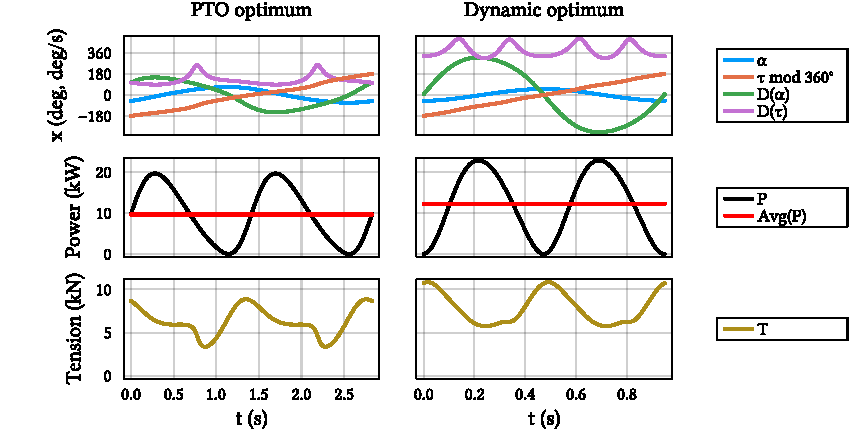
\includegraphics{figs/optimization_timeseries_all.pdf}
    \caption{Limit cycles for the initial guess (PTO optimum, left) and the optimized parameters (dynamic optimum, right): angles and angular velocities (top), instantaneous and average power (middle), line tension (bottom).
    The period goes from \SI{\PeriodInit}{\second} to \SI{\PeriodOpt}{\second}, and the average power increases by \(\PowerGain\%\).}
    \label{fig:time_series}
\end{figure}

\subsection{Optimal design as a function of wind speed} \label{sec:opt-wind}

Since the optimization converges quickly, we repeat the procedure for a range of reference wind speeds \(w_0\).
For each integer wind speed from \SIrange{\SweepWindMin}{\SweepWindMax}{\meter\per\second}, we find the set of parameters (Figure~\ref{fig:parameterized_optimization_params}) that maximizes power (Figure~\ref{fig:parameterized_optimization_power}) and show the corresponding minimum and maximum line tension over the limit cycle (Figure~\ref{fig:parameterized_optimization_tension}).
For comparison, we also compute the power and line tension extrema using the set of parameters obtained in Section~\ref{sec:opt-power}, optimized for a wind speed of \SI{\WindRef}{\meter\per\second}.
Over this whole range, this fixed set of parameters yields at most \(\SweepMaxLoss\%\) less power than the actual optimum, with a maximum line tension at most \(\SweepMaxTensionIncrease\%\) higher.
%\alter{landscape of the objective around the optimum: no asymmetry, just aim for the middle?}
The system exhibits quasilinear scaling along this parameterized optimization, even though the length of the arm (and other parameters) is kept constant, which makes it impossible to scale the model perfectly to wind speed.
Least-squares power laws along the optimized sweep give the following trends:
\begin{itemize}
    \item the average power grows like \(w_0^{\ExpPower}\), to be compared with the \(w_0^3\) scaling of wind power;
    \item the maximum line tension grows like \(w_0^{\ExpTension}\);
    \item the line length \(\ell\) and the arm inertia \(I\) vary as shown in Figure~\ref{fig:parameterized_optimization_params};
    \item the arm braking coefficient \(b\) grows like \(w_0^{\ExpBrake}\);
    \item (not shown) the period varies like \(w_0^{\ExpPeriod}\).
\end{itemize}

The maximum line tension defines the strength requirements for the kite fabric and lines.
Furthermore, the minimum line tension remains above \SI{\SweepMinTension}{\kilo\newton} over the whole sweep, confirming \emph{a posteriori} the modeling assumption that the lines are always in tension and never exert compression on the arm.

\begin{figure}[thpb]
  \centering
  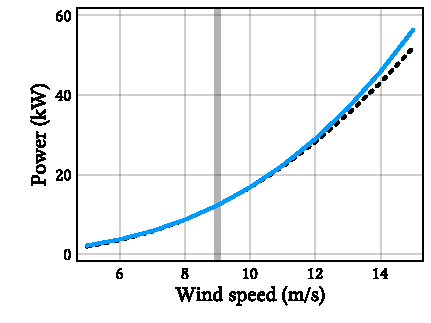
\includegraphics{figs/optimization_wind_sweep_power.pdf}
  \caption{Average generated power for optimized (blue) and reference (black) parameters when the reference wind speed \(w_0\) is varied.
  The reference curve is generated by fixing the design parameters to the optimal values for \(w_0 = \SI{\WindRef}{\meter\per\second}\).}
  \label{fig:parameterized_optimization_power}
\end{figure}

\begin{figure}[thpb]
  \centering
  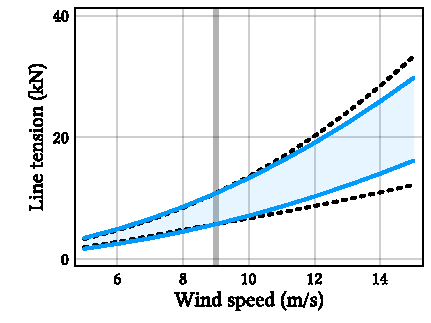
\includegraphics{figs/optimization_wind_sweep_tension.pdf}
  \caption{Minimum and maximum line tension \(\vb F_\ell\) for optimized (blue) and reference (black) parameters.}
  \label{fig:parameterized_optimization_tension}
\end{figure}

\begin{figure}[thpb]
  \centering
  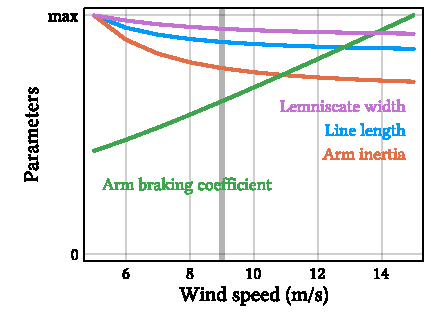
\includegraphics{figs/optimization_wind_sweep_params.pdf}
  \caption{Optimal parameters for each wind speed (color) and reference parameters fixed at the optimum for \(w_0 = \SI{\WindRef}{\meter\per\second}\) (black dashed lines).}
  % At this level of operation and despite relatively strong changes in the environmental parameter, the braking coefficient of the arm behaves linearly with respect to wind speed.
  \label{fig:parameterized_optimization_params}
\end{figure}

\subsection{Curvature of the kite trajectory} \label{sec:opt-curvature}

Besides power, a design has to be compatible with the flight of the kite: the turns of the curve \(t\mapsto\vb r(t)\) it describes must not be too strong.
We therefore derive upper bounds on the curvature \(\kappa\) of this curve; the computations and proofs are given in Appendix~\ref{app:curv}.

\paragraph{Setting.}
Recall that the kite position is \(\vb r = r\,\vu r(\tau)\), where \(\vu r\) is the spherical eight \eqref{eq:sphere_Model_Deriv}--\eqref{eq:traject_Model_Deriv}, a closed curve on the unit sphere with \(0<\theta_0-\Delta\theta\) and \(\theta_0+\Delta\theta<\pi\), and where \(r\) solves the line-length constraint:
\begin{equation}
    r = p + \sqrt{p^2+\ell^2-a^2}, \qquad p = a\,g, \qquad g = \sin\theta\cos(\phi-\alpha),
\end{equation}
so that \(\ell-a\le r\le\ell+a\), and \(r\equiv\ell\) when \(a=0\).
We write \(\varepsilon = a/\ell\) and \(\varepsilon' = a/\sqrt{\ell^2-a^2}\).
The kite trajectory is drawn on the \emph{cone} \(\mathscr C = \{r\,\vu r(\tau) : r>0,\ \tau\in\mathbf{S}^1\}\), the conical hull of the spherical eight.
Along a periodic orbit with \(\dot\tau\ne0\), the arm angle is a function \(\alpha(\tau)\), and since curvature does not depend on the parametrisation, the curvature \(\kappa = \norm{\vb r'\times\vb r''}/\norm{\vb r'}^3\) of the space curve (prime \(=\dv*{}{\tau}\)) does not depend on the time law \(\tau(t)\): \(\kappa(t) = \kappa(\tau(t))\).
It depends on \(\ell\), \(\Delta\theta\), \(\Delta\phi\), \(\theta_0\), \(a\), and on the arm law through \(\alpha,\alpha',\alpha''\); for \(a=0\), only on \(\ell,\Delta\theta,\Delta\phi,\theta_0\).

\paragraph{Curvature formula.}
Let \(v = \norm{\vu r'}\) be the speed on the sphere,
\begin{equation}
    v^2 = 4\Delta\theta^2\cos^22\tau + \Delta\phi^2\sin^2\theta\cos^2\tau > 0,
\end{equation}
\(\sigma(\tau) = \int_0^\tau v\) its arclength (so that \(f_\sigma = f'/v\) and \(f_{\sigma\sigma} = (f''v-f'v')/v^3\) for any function \(f\) of \(\tau\)), \(\vu t = \vu r_\sigma\) its unit tangent, \(\vu n = \vu r\times\vu t\), and \(\kappa_g\) its geodesic curvature on the sphere, defined by \(\vu t_\sigma = -\vu r + \kappa_g\vu n\):
\begin{equation} \label{eq:curv-kg}
    \kappa_g = \frac{2\Delta\theta\Delta\phi\sin\theta\,\sin\tau\,(2+\cos2\tau) + \Delta\phi\cos\theta\cos\tau\,\bigl(8\Delta\theta^2\cos^22\tau + \Delta\phi^2\sin^2\theta\cos^2\tau\bigr)}{v^3}.
\end{equation}
Finally let \(u = \ln r\).
For every \(\tau\),
\begin{equation} \label{eq:curv-formula}
    r\,\kappa = \frac{\sqrt{\kappa_g^2\,(1+u_\sigma^2) + (1+u_\sigma^2-u_{\sigma\sigma})^2}}{(1+u_\sigma^2)^{3/2}}.
\end{equation}
The cone \(\mathscr C\) is a developable surface, with principal curvatures \(0\) along the generators and \(\kappa_g/r\) across them.
Formula \eqref{eq:curv-formula} is the decomposition \(\kappa^2 = \kappa_n^2 + (\kappa_g^{\mathscr C})^2\) of the curvature of a curve drawn on \(\mathscr C\) into its normal and geodesic parts:
\begin{equation}
    \kappa_n = \frac{\kappa_g}{r}\sin^2\beta = \frac{\kappa_g}{r\,(1+u_\sigma^2)}, \qquad \kappa_g^{\mathscr C} = \frac{1+u_\sigma^2-u_{\sigma\sigma}}{r\,(1+u_\sigma^2)^{3/2}},
\end{equation}
where \(\beta\) is the angle between the trajectory and the generator.
The normal part is controlled by the curvature of the surface, \(\abs{\kappa_n}\le\abs{\kappa_g}/r\), and is entirely due to the bending of the spherical eight; the geodesic part is the curvature of the planar polar curve \(\sigma\mapsto r(\sigma)\) obtained by unrolling the cone, and is due to the variation of \(r=\norm{\vb r}\) along the cycle.
The surface therefore bounds \(\kappa\) from below only, by \(\abs{\kappa_n}\); this lower bound vanishes at the inflection points of the eight, where \(\kappa_g=0\), and it gives no upper bound.

\paragraph{Without arm.}
For \(a=0\), the trajectory lies on the sphere of radius \(\ell\), the unrolled curve is a circle of radius \(\ell\), and
\begin{equation}
    \kappa = \frac{\sqrt{1+\kappa_g^2}}{\ell} \ \ge\ \frac1\ell,
\end{equation}
with equality at the inflection points of the eight, which exist on each lobe.
In particular, the floor \(1/\ell\) is a property of the trajectory in the cone, not of the cone.
Large curvature is produced where the spherical eight turns sharply, \emph{i.e.} where \(v\) is small compared with the bending of the eight: at the lobe tips \(\tau=\pi/2,3\pi/2\) for a wide eight (\(\Delta\theta\) small compared with \(\Delta\phi\sin\theta_0\)), and at the top and bottom \(\tau=\pi/4,3\pi/4\) for a tall eight.
Indeed, exactly,
\begin{equation}
    \kappa_g(\pi/2) = \frac{\Delta\phi\sin\theta_0}{4\Delta\theta^2}, \qquad
    \kappa_g(3\pi/4) = \frac{8\Delta\theta}{\Delta\phi^2\sin^2(\theta_0-\Delta\theta)} - \cot(\theta_0-\Delta\theta),
\end{equation}
so that, for \(a=0\), \(\max\kappa\to\infty\) as \(\Delta\theta\to0\) or as \(\Delta\phi\to0\), the other parameters being fixed.

\paragraph{Upper bound.}
Consider a box of parameters: let \(\ell\ge\ell_->a\), \(\Delta\theta\in[\Delta\theta_-,\Delta\theta_+]\), \(\Delta\phi\in[\Delta\phi_-,\Delta\phi_+]\) with \(\Delta\theta_->0\), \(\Delta\phi_->0\), and \(\theta_0\in[\theta_{0-},\theta_{0+}]\) with \(\mathscr J = [\theta_{0-}-\Delta\theta_+,\ \theta_{0+}+\Delta\theta_+]\subset(0,\pi)\).
Set
\begin{equation}
    m = \min_{\mathscr J}\sin, \qquad M = \max_{\mathscr J}\sin, \qquad C = \max_{\mathscr J}\abs{\cos},
\end{equation}
\begin{equation}
    v_* = \begin{cases}
        2\Delta\theta_- & \text{if } m\Delta\phi_-\ge4\Delta\theta_-, \\[2pt]
        m\Delta\phi_-\sqrt{\dfrac12 - \dfrac{m^2\Delta\phi_-^2}{64\,\Delta\theta_-^2}} & \text{otherwise,}
    \end{cases}
    \qquad
    \bar\kappa_g = \frac{2\sqrt2\,M\,\Delta\theta_+\Delta\phi_+}{v_*^3} + \frac{2C}{m}.
\end{equation}
Let the arm law satisfy \(\abs{\alpha'}\le A_1\) and \(\abs{\alpha''}\le A_2\), and set
\begin{equation}
\begin{split}
    &\Gamma_1 = 2\Delta\theta_+ + \Delta\phi_+ + A_1, \qquad \Gamma_2 = \Gamma_1^2 + 4\Delta\theta_+ + \Delta\phi_+ + A_2, \\
    &V_1 = 4\Delta\theta_+ + \Delta\phi_+ + \tfrac12\Delta\phi_+^2 + 4\Delta\theta_+\Delta\phi_+, \qquad
    U = \varepsilon'\,\frac{\Gamma_2 + \varepsilon'^2\,\Gamma_1^2}{v_*^2} + \varepsilon'\,\frac{\Gamma_1V_1}{v_*^3}.
\end{split}
\end{equation}
Then, for all parameters in the box, every such arm law, and every \(\tau\),
\begin{equation} \label{eq:curv-bound}
    \kappa \le \frac{\sqrt{\bar\kappa_g^2 + (1+U)^2}}{\ell_--a},
\end{equation}
and, without arm (\(a=0\), \(U=0\)), \(1/\ell\le\kappa\le\sqrt{1+\bar\kappa_g^2}/\ell_-\).
Since \(U = O(\varepsilon)\), the bound is \(\sqrt{1+\bar\kappa_g^2}/\ell_- + O(\varepsilon)\), uniformly on the box.
The bound degenerates only when \(\Delta\theta_-\to0\), \(\Delta\phi_-\to0\), or \(\mathscr J\) reaches a pole, which is unavoidable by the exact tip and bottom values above; and, when \(a>0\), the bound on \(\alpha''\) cannot be dispensed with, since \(u_{\sigma\sigma}\), which contains \(\alpha''\) linearly, enters \eqref{eq:curv-formula} through \(\abs{1+u_\sigma^2-u_{\sigma\sigma}}\).
In the optimization above, the lower bound on \(\ell\) in Table~\ref{tab:opt_descr} plays the role of \(\ell_-\), while \(A_1\) and \(A_2\) can be evaluated on the computed periodic orbits.

\paragraph{First order in the arm length.}
With \(K = \sqrt{1+\kappa_g^2}\), for a fixed eight and a fixed arm law with bounded \(\alpha',\alpha''\),
\begin{equation} \label{eq:curv-first-order}
    \ell\,\kappa = K\,(1-\varepsilon g) - \varepsilon\,\frac{g_{\sigma\sigma}}{K} + O(\varepsilon^2)
\end{equation}
uniformly in \(\tau\): the arm rescales the arm-free curvature by \(\ell/r\) and adds the contribution of the second derivative of \(g\) (hence of \(\alpha''\)) along the eight.

\paragraph{Example (without arm).}
For the optimized eight of Table~\ref{tab:opt_results} (\(\Delta\theta=\DthetaFixed^\circ\), \(\Delta\phi=\DphiOpt^\circ\), \(\theta_0=\ThetaZero^\circ\)), the exact value above gives \(\kappa_g(\pi/2)\simeq\CurvTipKg\), hence \(\ell\kappa(\pi/2) = \sqrt{1+\kappa_g(\pi/2)^2} \simeq \CurvTipK\) at the lobe tips for \(a=0\).
This value at the tip is exact: it follows from the formulas above, with no approximation.
The tips are not necessarily where the turn is sharpest: sampling \(\tau\) on a fine grid gives \(\max_\tau\ell\kappa\simeq\CurvMaxK\), reached at \(\tau\simeq\CurvMaxTau\) and, by symmetry, at \(\tau+\pi\); the smallest radius of curvature of the trajectory is thus about \(\ell/\CurvMaxK\), \emph{i.e.} about \SI{\CurvMaxRadius}{\meter} for the optimized length \(\ell=\SI{\EllOpt}{\meter}\).
The case \(a>0\) was not examined here; there, only the upper bound \eqref{eq:curv-bound} is proven.


\begin{table}[htbp]
  \centering
  \caption{Comparison of initial and optimized parameters}
  \label{tab:parameter_comparison}
  \begin{tabular}{lrr}
    \toprule
    Parameter & \multicolumn{1}{c}{PTO initialization} & \multicolumn{1}{c}{Dynamic ptimization} \\
    \midrule
    $\ell$ ($\mathrm{m}$)                             & 31.0     & 26.9679  \\
    $I$ ($\mathrm{kg\cdot m^2}$)                     & 1300.0   & 351.628  \\
    $b$ ($\mathrm{kg\cdot m^2\cdot s^{-1}\cdot rad^{-1}}$) & 2888.29  & 737.073  \\
    $\Delta\phi$ ($\mathrm{rad}$)                    & 0.872665 & 0.29     \\
    \midrule
    Period ($\mathrm{s}$)                            & 2.82807  & 0.949268 \\
    Objective $P$ ($\mathrm{kW}$)                    & 9.63887  & 12.2534  \\
    Min tension ($\mathrm{kN}$)                      & 3.35552  & 5.74767  \\
    Max tension ($\mathrm{kN}$)                      & 8.85567  & 10.8269  \\
    Max acceleration ($\mathrm{m/s^2}$)              & 517.078  & 938.602  \\
    \bottomrule
  \end{tabular}
\end{table}



\begin{figure}[thpb]
    \centering
        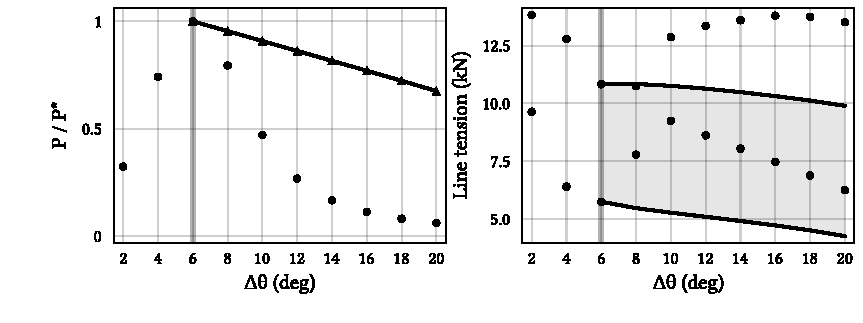
\includegraphics{figs/optimization_dtheta.pdf}
    \caption{Average power and line tension and acceleration as $\Delta \theta$ varies. 6° gives a good combination of average power (higher is better) and line tension (lower is better).}
    \label{fig:opt-dtheta}
\end{figure}

\begin{figure}[thpb]
    \centering
    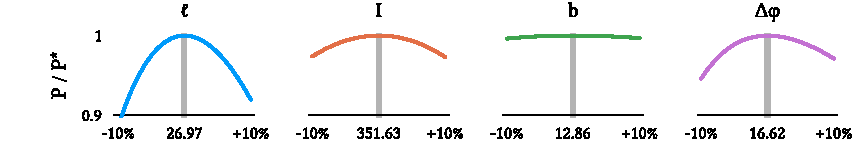
\includegraphics{figs/optimization_landscape.pdf}
    \caption{Average power as the optimization parameters vary.
    % TODO which variables are on their bounds? which variables have the most impact? could reoptimize other 3 parameters
    The objective landscape is smooth, explaining the easy numerical solving.}
    \label{fig:opt-landscape}
\end{figure}
